\documentclass{acm_proc_article-sp}
\usepackage{graphicx}
\def\url#1{{\tt#1}}

\begin{document}

\title{The summary title}

\numberofauthors{3} 
\author{
\alignauthor
Jakub Marou\v sek
       \email{jakub.marousek@gmail.com}%
% put your details here
}

\maketitle
\begin{abstract}
Place an abstract here.
\end{abstract}

\section{Introduction}

\cite{braams:babel}

\section{The {\secit Body} of The Paper}

\subsection{Introduction to ext4}

The ext4 filesystem is the next generation in the family of ext filesystems, used typically in Linux environments. In the very beginning, the Linux kernel used Minix filesystem, due to the fact that Linux itself originated from Minix. This filesystem, however, contained serious limitations, the maximum file name size and the maximum filesystem size as the most severe examples. A group of kernel developers, with Theodore Ts'o being the most prominent one, introduced a couple of new filesystems \cite{ext2design}.

The first new filesystem, ext (``extended file system'', released in 1992) removed the Minix limitations, but some of the previous problems remained -- for example, free blocks were monitored over a linked list, which harmed performance. As a quick response, ext2 (``second extended file system'', 1993) was released. While the code of ext2 originated in that of ext, it brought many notable improvements.

\subsubsection{The ext2 filesystem}

The filesystem supports standard Unix file types: regular files, directories, device-special files and links. The maximum size of a file is 2 GB, the maximum size of the whole filesystem is 4 TB.
As the other Unix filesystems, it also uses inodes for storing file metadata. An {\it inode} is a structure containing a description of a file: file type, access rights, owners, timestamps, size, pointers to data blocks.

A directory is only a special kind of file, with a list of files and their corresponding inodes. A link can be either hard or symbolic. A hard link is basically a file pointing to the same inode as the original file, not distinguishable from the previous file. To remove a hard-linked file, all the references to the file must be removed. A symbolic link contains a text specifying a path to the file. Unlike the symlink, creating a hard link has limitations: it is possible to hard-link only a file from the same partition (due to the nature of the link) and hard-linking directories is not allowed (to prevent infinite subdirectory loops). A device-special file is only a pointer to the device driver.

While these features are common for all Unix filesystems, now we shall list some abilities specifical for ext2. Using the file attributes, the kernel behavior of creating new files in a directory can be modified, specifically the new file user id and group id. The logical block sizes can be specified when the filesystem is created -- larger block sizes lead to efficient behavior, but also wastes more space.

The symbolic links of ext2 can use more efficient way of storing the path inside the inode of the symlink. The overall status of the filesystem is saved in the superblock. During the mounting of the filesystem, if it is detected that it was not unmounted properly, the filesystem is automatically checked. After a certain number of mounts or when a certain time period has passed, the filesystem checking is enforced.

It is also possible to create {\it immutable} files, which either cannot be written into or deleted, or they can be opened for writing, but the text is appended to the end of the file.

\begin{figure}
\centering
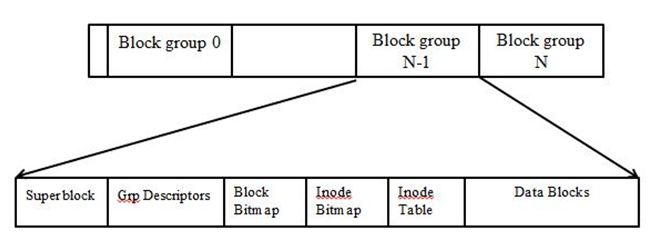
\includegraphics[width=0.48\textwidth]{images/ext2structure.jpg}
	\caption{The structure of an ext2 filesystem \cite{ext2structure}}
\end{figure}

{\bf The filesystem structure} is as follows. There is a boot sector in the beginning of the space, which is designated for bootloaders code. The rest of the drive is split into {\it block groups}. Each block groups contains inodes (in an inode table) and data blocks. An inode bitmap and a block bitmap marks which inode/block is used and which is not. 

The superblock and group descriptors contain information which are crucial for the filesystem functioning, and thus they are put in the beginning of each group as a backup. The superblock contains the basic information about the structures, like logical block sizes, the number of blocks and inodes, positions of data blocks and so on. An array of group descriptors contains pointers to the inode table and the block table for every present group.

As the main optimization, ext2 performs block readahead, that means, reads more continguous blocks at once. Block groups try to keep together inodes and blocks of a file, which reduces disk seeks. Also when a file is being written, ext2 preallocates up to 8 blocks.

\subsubsection{The ext3 file system}

After the initial period of bugs elimination, the ext2 file system has become a safe, stable choice for a Linux-based operating system. One of the main drawbacks of using ext2 is the lack of jounrnaling, which slows down the file system check and makes files prone to corruption.

First suggestions for the journaling of ext file system family were put down by Stephen C.\ Tweedie \cite{extjournal}. He identifies several aspects of file system reliability and puts forward {\it preservation} (``stable'' data on the disk should never be damaged), {\it predictability} (the failure modes of the file system should be predictable and deterministic) and {\it atomicity} (every operation is either fully performed or fully undone). The ext2 provided only the preservation aspect, whilst the failure states (could occur because of an unexpected reboot, for example) were not properly defined and might have prevented the operations from fully performing.

The Tweedie's article \cite{extjournal} compares approaches of reaching the desired aspects. The easiest way is to wait for a disk write to complete before the next one is submitted, which breaks the performance. Another idea lies in preserving multiple write buffers, ordering them accordingly and write these separately. However, one can easily get into a situation when the buffer dependendence is cyclic (moving a file from directory $A$ to directory $B$ and, in the same time, moving another file from $B$ to $A$). While there exists a mechanism to solve it, all the presented approaches require the disk to be completely rescanned for errors in case of a system failure. (Recall that file system check slowness was one of main objections against ext2.)

Instead, the author proposes to use {\it journaling}. To ensure operations to be atomic, a batch of data is written on the disk, but is not effective until a special {\it commit} block does not conclude the operation. Thus, a failure during performing the write can result only in two possibilities: either the commit block has been written on the disk, which means the transaction is complete, or it has not been written, in which case the transaction as a whole is undone. More practically: there is a dedicated place on the disk, called a {\it journal}, working as a cycling buffer. A transaction starts with a description block, continues with all the blocks that the transaction is modifying, and end with a commit block. Only after all these blocks have been successfully written to the journal, the ``real'' blocks modification is done. If a failure of the system occurs, the recovery program goes through the journal and performs all transactions which contain the commit block. If the block is not present, the transaction is discarded.

\begin{figure}
\centering
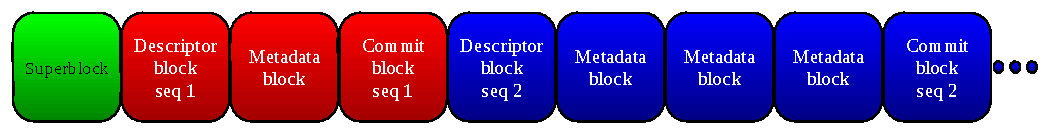
\includegraphics[width=0.48\textwidth]{images/journal.pdf}
	\caption{The structure of ext3 journal \cite{takingadvantage}}
\end{figure}

The ext3 file system, released in 2001, i offers three different modes of journaling: \cite{takingadvantage}

\begin{itemize}
	\item {\it Journal} -- All data and matadata are logged. This approach minimizes the chance of losing data, but has the laregst performance penalty.
	\item {\it Ordered} -- Only metadata are logged, but file data are flushed on the disk before the change of metadata occurs, keeping the journal synchronized with data writes. This is the default mode.
	\item {\it Write back} -- Only metadata are logged, file data are flushed whenever possible. This mode is the fastest, but also the most dangerous.
\end{itemize}

Notice that journaling cannot be turned off. Compared to ext2, this is the only different feature. Thanks to this, it is possible to convert an ext2 partition to ext3 with spawning a single command.
For the period of ext3 development, a principle of both backward and forward compatibility with ext2 was closely followed by its authors. Therefore, an ext3 partition can be mounted with ext2 driver and works the same with the exception of journaling. Turning off a journal causes an ext3 partition to become ext2 and vice versa.

\subsubsection{The ext4 file system}

Although ext3 was a step forward, it still lacked some state-of-the-art features, which could be found in other Unix filesystems. Between 2003 and 2006, numberous patches for the ext3 were proposed to be added to the Linux kernel, but they were not accepted because the Linux community was afraid of stability of their mostly-used-file system at that time. As a result, Theodore Ts'o introducted plans for creating a successor of ext3, which would partially break the forward compatibility, but still allowed an easy update from the older versions \cite{newext4}. In 2008, the code was marked as stable.

A large amount work was done in terms of scalability. The maximum size of the file system was raised to 1 EB, the maximum size of a file is raised to 2 TB. The maximum number of files is increased too.

A compatibility-breaking change of file block locations is brought up. Instead of storing a list of data blocks (which is advantageous for small files but unpractical for large ones), {\it extents} are introduced. An extent is a range of data blocks, where all blocks in the range belong to the file. Four extents can be directly stored in the inode of the file. For large and fragmented files, a tree of pointers is maintained, with extents being in the leaves.

\begin{figure}
\centering
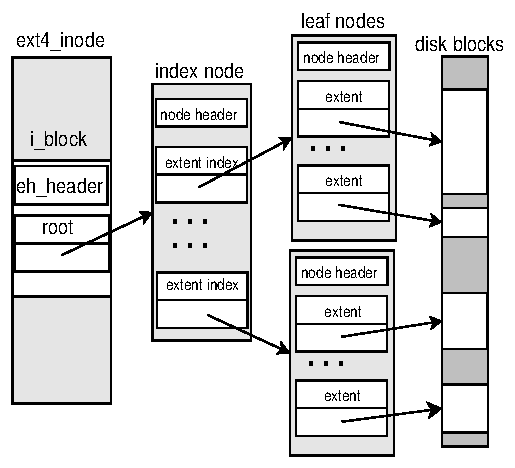
\includegraphics[width=0.48\textwidth]{images/extents.pdf}
	\caption{Extent tree layout \cite{newext4}}
\end{figure}

The transactions in the journal are checksummed in the commit block, making two consequences: the recovery is more reliable as the corrupted transaction blocks are detected and the transaction cancelled; also now the commit block can be written in the same time as the other blocks, which significantly improves the performance.

Contrary to ext4, persistent pre-allocation of file size is possible. The checking of the file system is 2 to 20 times 2 to 20 times faster, as the unallocated inodes are marked and are skipped during the rest of the procedure. Instead of allocating one block at a time, the allocation is {\it delayed} in ext4, meaning it is postponed in time and performed when the file is flushed. There is also a possibility of online defragmentation. Since the size of an inode is larger, nanosecond resolution timestamps are supported and the problem of year 2038 is deferred for 272 years.

Similarly as in the case of ext2 and ext3, migrating to ext4 is just a matter of turning on the new features. The legacy system of individual block mapping is preserved, but all new files will use extents. Downgrading from ext4 to ext3 by turning off the features is straightforward when extents are not used -- otherwise, temporary copy of the files is needed.

\subsubsection{Comparison of ext4 and other Unix file systems}

It is worth noting that Theodore Ts'o considered ext4 not to be a major advance and still using old technology. In the light of his words, I found potentially interesting to list other popular Unix filesystems and compare their functions.

{\it Btrfs} \cite{btrfs} is a file system brought to life by Oracle. The development began in 2007 and the software was proclaimed to be stable in 2014. The name comes from the B-tree as this is the main structure used within the file system. Notable features of Btrfs are copy-on-write (a copied and unmodified file references to the ``old data''), snapshots, CRC checksums of data, RAID or configurable compression. In order to prolong the lifespan, SSD drivers are handled specifically. In-place conversion from ext2/3/4 and ReiserFS is present.

{\it ReiserFS} was created by company Namesys with Hans Reiser as the chief developer. When the first version was released in 2001, it brought attention because of features which had been unavailable, like journaling, online filesystem resizing, packing files in a single disk block or B-tree usage. Although ReiserFS was popular in the past, it was overtaken by other file systems since then. The main reason may be the slow pace of development, especially after Hans Reiser has been imprisoned and convicted of murder.

{\it ZFS} \cite{zfs} was developed by Oracle, but after the end of support the project was handled to the open-source community \cite{openzfs}. It supports journaling, read-only snaphots of the files state, RAID or checksums of files. On Ubuntu, ZFS has been chosen as the default filesystem for containers.

\subsection{Files carving}

\subsection{Related works}

\section{Conclusions}

\bibliographystyle{abbrv}
\bibliography{paper}

\balancecolumns
\end{document}
